\documentclass[tikz,border=4pt]{standalone}
\usepackage{ctex}\usepackage{pgfplots}\pgfplotsset{compat=1.18}
\begin{document}
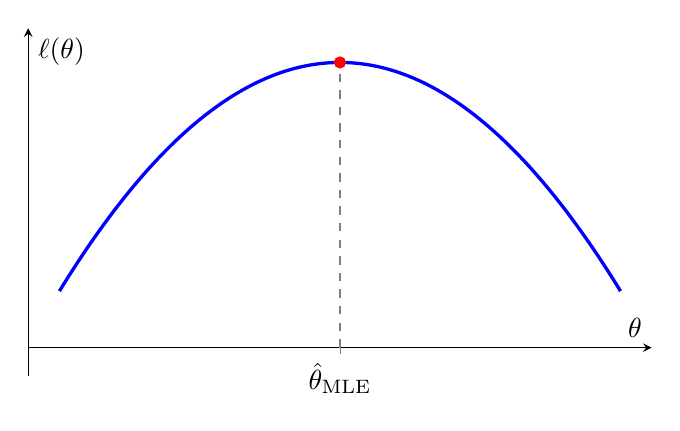
\begin{tikzpicture}
\begin{axis}[axis lines=middle,xlabel={$\theta$},ylabel={$\ell(\theta)$},xmin=0,xmax=6,ymin=-0.5,ymax=5.6,width=9.5cm,height=6cm,xtick={3},xticklabels={$\hat{\theta}_{\mathrm{MLE}}$},ytick=\empty,samples=120]
\addplot[blue,very thick,domain=0.3:5.7]{5-(x-3)^2*0.55};
\draw[dashed,gray](axis cs:3,0)--(axis cs:3,5);
\addplot[only marks,red,mark=*]coordinates{(3,5)};
\end{axis}
\end{tikzpicture}
\end{document}
